\documentclass[12pt,a4paper]{article}
\usepackage[margin=1in, includeheadfoot]{geometry}
\usepackage{mathptmx}
\usepackage{booktabs}
\usepackage{longtable}
\usepackage{array}
\usepackage{hyperref}
\usepackage{titlesec}
\usepackage{fancyhdr}
\usepackage{graphicx}
\usepackage{parskip}
\usepackage{tabularx}
\usepackage{microtype}
\usepackage{tikz}
\usepackage{eso-pic}
\usepackage{xcolor}
\usepackage{float}

\hypersetup{colorlinks=false, hidelinks}

\AddToShipoutPictureBG{%
  \begin{tikzpicture}[overlay, remember picture]
    \draw[line width=1.5pt, color=black!70]
      ([xshift=15pt, yshift=-15pt]current page.north west)
      rectangle
      ([xshift=-15pt, yshift=15pt]current page.south east);
  \end{tikzpicture}%
}

\titleformat{\section}{\large\bfseries}{}{0em}{}[\titlerule\vspace{-4pt}]
\titlespacing{\section}{0pt}{10pt}{8pt}
\titleformat{\subsection}{\normalsize\bfseries}{}{0em}{}
\titlespacing{\subsection}{0pt}{8pt}{4pt}

\pagestyle{fancy}
\fancyhf{}
\cfoot{\thepage}
\renewcommand{\headrulewidth}{0pt}

\setlength{\parskip}{4pt}
\setlength{\parindent}{0pt}
\setlength{\extrarowheight}{3pt}

\newcolumntype{L}[1]{>{\raggedright\arraybackslash}p{#1}}

\begin{document}

%----------------------------------------------------------
% TITLE PAGE
%----------------------------------------------------------
\begin{titlepage}
\AddToShipoutPictureBG*{%
  \begin{tikzpicture}[overlay, remember picture]
    \draw[line width=2pt, color=black!80]
      ([xshift=15pt, yshift=-15pt]current page.north west)
      rectangle
      ([xshift=-15pt, yshift=15pt]current page.south east);
    \draw[line width=0.6pt, color=black!40]
      ([xshift=20pt, yshift=-20pt]current page.north west)
      rectangle
      ([xshift=-20pt, yshift=20pt]current page.south east);
  \end{tikzpicture}%
}
    \centering
    \includegraphics[width=8cm]{cmd.png}\\[0.3cm]
    {\large \textbf{Bahria University}}\\[0.1cm]
    {\small Department of Computer Science}\\[0.4cm]
    \rule{\linewidth}{0.5mm}\\[0.3cm]
    {\LARGE \textbf{Skill Barter Platform}}\\[0.3cm]
    \rule{\linewidth}{0.5mm}\\[0.5cm]
    \begin{tabular}{ll}
        \textbf{Submitted to:} & Aima Zahoor \\
        \textbf{Semester:}     & Spring 2026 \\
        \textbf{Class:}        & BS-CS 4-B \\
        \textbf{Deadline:}     & May 10, 2026 \\
    \end{tabular}\\[0.6cm]
    \textbf{Group Members}\\[0.3cm]
    \begin{tabular}{cll}
        \toprule
        \textbf{Sr.} & \textbf{Name} & \textbf{Enrollment No.} \\
        \midrule
        1 & Muhammad Sadiq Aslam Khan & 01-134242-091 \\
        2 & Malik Junaid Ahmed        & 01-134242-061 \\
        3 & Bilawal Khokhar           & 01-134242-036 \\
        4 & Shah Murad                & 01-134242-113 \\
        \bottomrule
    \end{tabular}
    \vfill
    {\small May 2026}
\end{titlepage}

\tableofcontents
\newpage

%##########################################################
%  MILESTONE 1
%##########################################################
\begin{center}
{\LARGE \textbf{Milestone 1: Requirements}}\\[0.1cm]
\rule{\linewidth}{0.6mm}
\end{center}
\vspace{4pt}

\section{Problem Statement}
\vspace{4pt}

Students, freelancers, and working professionals often need new skills but cannot afford paid tutoring or courses. At the same time, plenty of people have skills they would teach but no way to find someone who wants to learn them.

A skill barter platform fixes this by letting users swap skills directly. Someone who knows web development and wants to learn graphic design finds another user with the opposite setup and arranges a trade. No money changes hands. The system handles matching, messaging, scheduling, and feedback so users do not have to sort it out themselves.

Every existing option is either a paid platform, a disorganised social media group, or a freelance marketplace built around money. Nothing is built specifically around skill exchange.

\section{Project Scope}
\vspace{4pt}

Users can register, build profiles, and list skills they offer and skills they want. The system matches users with complementary skill sets. Users send and receive barter requests, communicate through a messaging interface, and schedule sessions. After a session, both parties rate each other. Admins manage users, resolve disputes, and monitor platform activity.

The system does not handle payments, real-time video calls, or third-party login. Hardware integration is out of scope. The platform is documented as a web-based application.

\section{Functional Requirements}
\vspace{4pt}

\begin{longtable}{>{\bfseries}p{1.8cm} p{11.5cm}}
\toprule
\textbf{FR ID} & \textbf{Requirement} \\
\midrule
\endfirsthead
\toprule
\textbf{FR ID} & \textbf{Requirement} \\
\midrule
\endhead
\bottomrule
\endfoot
FR-01 & Users can register with name, email, and password \\
FR-02 & Users can log in and log out securely \\
FR-03 & Users can create and edit their profile including skills offered and skills wanted \\
FR-04 & Users can search and browse other users by skill \\
FR-05 & Users can send a barter request to another user \\
FR-06 & Users can accept or reject incoming barter requests \\
FR-07 & Matched users can communicate through an in-platform messaging system \\
FR-08 & Users can schedule a session with date, time, and mode (online or in-person) \\
FR-09 & Users can rate and review each other after a completed session \\
FR-10 & Users can view their barter history \\
FR-11 & Admin can view, suspend, or delete any user account \\
FR-12 & Admin can view all active and completed barter sessions \\
FR-13 & Admin can resolve reported disputes between users \\
FR-14 & Users can report another user for misconduct \\
FR-15 & System sends notifications for new requests, messages, and session reminders \\
\end{longtable}

\section{Non-Functional Requirements}
\vspace{4pt}

\begin{longtable}{>{\bfseries}p{1.8cm} p{3.2cm} p{8.3cm}}
\toprule
\textbf{NFR ID} & \textbf{Category} & \textbf{Requirement} \\
\midrule
\endfirsthead
\toprule
\textbf{NFR ID} & \textbf{Category} & \textbf{Requirement} \\
\midrule
\endhead
\bottomrule
\endfoot
NFR-01 & Performance     & Search results load within 2 seconds under normal load \\
NFR-02 & Scalability     & System supports up to 10,000 concurrent users \\
NFR-03 & Security        & Passwords are stored as hashed values, never plain text \\
NFR-04 & Security        & Role-based access control separates user and admin functions \\
NFR-05 & Usability       & New users can register and send a barter request within 5 minutes \\
NFR-06 & Availability    & System uptime is 99.5\% or higher \\
NFR-07 & Maintainability & System uses a layered architecture so modules can be updated independently \\
NFR-08 & Reliability     & All barter request state changes are logged and recoverable \\
NFR-09 & Compatibility   & Platform is accessible on modern web browsers without plugins \\
NFR-10 & Privacy         & User personal data is not visible to other users without consent \\
\end{longtable}

\newpage
\section{Use Case Diagram}
\vspace{4pt}

\textbf{Actors:} Registered User, Admin, Notification Service (external)

\textbf{Use Cases:} Register/Login, Manage Profile, Search Users by Skill, Send Barter Request, Accept/Reject Request, Message Matched User, Schedule Session, Rate and Review, View Barter History, Report User, Manage Users (Admin), Resolve Dispute (Admin), View Platform Reports (Admin), Send Notifications (Notification Service)

\begin{figure}[H]
\centering
\includegraphics[page=13, width=\textwidth]{diagrams.pdf}
\end{figure}

\newpage
\section{Use Case Description Tables}
\vspace{4pt}

\subsection*{UC-01: Register / Login}
\begin{longtable}{>{\bfseries}L{3.5cm} L{10cm}}
\toprule
\textbf{Field} & \textbf{Description} \\ \midrule \endfirsthead \midrule \textbf{Field} & \textbf{Description} \\ \midrule \endhead \bottomrule \endfoot
Use Case ID      & UC-01 \\
Actor            & Registered User \\
Description      & New user creates an account. Existing user logs in with credentials. \\
Preconditions    & User has browser access to the platform \\
Normal Flow      & 1. User opens platform. 2. New user fills name, email, password and registers. 3. Existing user enters credentials and logs in. 4. System redirects to dashboard. \\
Alternative Flow & If email is already registered, system prompts login instead. \\
Exception Flow   & After 3 failed login attempts, account is locked temporarily. \\
Postconditions   & User is authenticated and can access platform features. \\
\end{longtable}

\subsection*{UC-02: Manage Profile}
\begin{longtable}{>{\bfseries}L{3.5cm} L{10cm}}
\toprule
\textbf{Field} & \textbf{Description} \\ \midrule \endfirsthead \midrule \textbf{Field} & \textbf{Description} \\ \midrule \endhead \bottomrule \endfoot
Use Case ID      & UC-02 \\
Actor            & Registered User \\
Description      & User creates or updates profile with bio, skills offered, and skills wanted. \\
Preconditions    & User is logged in \\
Normal Flow      & 1. User goes to profile page. 2. Edits bio and skill lists. 3. Saves changes. 4. System updates profile. \\
Alternative Flow & Multiple skills can be added in both categories. \\
Exception Flow   & Required fields left empty prompt user before saving. \\
Postconditions   & Profile is updated and searchable by other users. \\
\end{longtable}

\subsection*{UC-03: Search Users by Skill}
\begin{longtable}{>{\bfseries}L{3.5cm} L{10cm}}
\toprule
\textbf{Field} & \textbf{Description} \\ \midrule \endfirsthead \midrule \textbf{Field} & \textbf{Description} \\ \midrule \endhead \bottomrule \endfoot
Use Case ID      & UC-03 \\
Actor            & Registered User \\
Description      & User searches for other users who offer a specific skill. \\
Preconditions    & User is logged in and other users have skills listed \\
Normal Flow      & 1. User enters skill in search bar. 2. System returns matching users. 3. User views profiles. \\
Alternative Flow & Results can be filtered by rating or availability. \\
Exception Flow   & No matching results shows a no results message. \\
Postconditions   & User views profiles and can send a barter request. \\
\end{longtable}

\subsection*{UC-04: Send Barter Request}
\begin{longtable}{>{\bfseries}L{3.5cm} L{10cm}}
\toprule
\textbf{Field} & \textbf{Description} \\ \midrule \endfirsthead \midrule \textbf{Field} & \textbf{Description} \\ \midrule \endhead \bottomrule \endfoot
Use Case ID      & UC-04 \\
Actor            & Registered User \\
Description      & User sends a barter request proposing a skill exchange to another user. \\
Preconditions    & User is logged in and has at least one skill listed \\
Normal Flow      & 1. User views another profile. 2. Clicks Send Barter Request. 3. Selects skill offered and skill wanted. 4. Adds optional message and submits. 5. Recipient is notified. \\
Alternative Flow & Request can be edited before submitting. \\
Exception Flow   & No skill listed prompts user to update profile first. \\
Postconditions   & Request created with pending status and recipient notified. \\
\end{longtable}

\subsection*{UC-05: Accept or Reject Request}
\begin{longtable}{>{\bfseries}L{3.5cm} L{10cm}}
\toprule
\textbf{Field} & \textbf{Description} \\ \midrule \endfirsthead \midrule \textbf{Field} & \textbf{Description} \\ \midrule \endhead \bottomrule \endfoot
Use Case ID      & UC-05 \\
Actor            & Registered User \\
Description      & User reviews an incoming barter request and accepts or rejects it. \\
Preconditions    & User has at least one pending incoming request \\
Normal Flow      & 1. User opens request inbox. 2. Views request details. 3. Clicks Accept or Reject. 4. Sender is notified. \\
Alternative Flow & User can send a message before deciding. \\
Exception Flow   & None. \\
Postconditions   & If accepted, both users proceed to messaging and scheduling. \\
\end{longtable}

\subsection*{UC-06: Schedule Session}
\begin{longtable}{>{\bfseries}L{3.5cm} L{10cm}}
\toprule
\textbf{Field} & \textbf{Description} \\ \midrule \endfirsthead \midrule \textbf{Field} & \textbf{Description} \\ \midrule \endhead \bottomrule \endfoot
Use Case ID      & UC-06 \\
Actor            & Registered User \\
Description      & Matched users agree on a date, time, and mode for the skill exchange session. \\
Preconditions    & Barter request has been accepted \\
Normal Flow      & 1. Either user opens the barter thread. 2. Proposes date, time, and mode. 3. Other user confirms. 4. System records session and sends reminders. \\
Alternative Flow & Users can reschedule before the session date. \\
Exception Flow   & No confirmation within 7 days marks the session as expired. \\
Postconditions   & Session is scheduled and both users receive reminders. \\
\end{longtable}

\subsection*{UC-07: Rate and Review}
\begin{longtable}{>{\bfseries}L{3.5cm} L{10cm}}
\toprule
\textbf{Field} & \textbf{Description} \\ \midrule \endfirsthead \midrule \textbf{Field} & \textbf{Description} \\ \midrule \endhead \bottomrule \endfoot
Use Case ID      & UC-07 \\
Actor            & Registered User \\
Description      & After a completed session, both users rate each other and leave an optional review. \\
Preconditions    & Session has been marked as completed \\
Normal Flow      & 1. System prompts both users to rate. 2. User gives 1 to 5 stars and optional written review. 3. System saves and displays on profile. \\
Alternative Flow & User can skip written review and submit rating only. \\
Exception Flow   & Rating window closes after 7 days if not submitted. \\
Postconditions   & Rating recorded and profile score updated. \\
\end{longtable}

\subsection*{UC-08: Report User}
\begin{longtable}{>{\bfseries}L{3.5cm} L{10cm}}
\toprule
\textbf{Field} & \textbf{Description} \\ \midrule \endfirsthead \midrule \textbf{Field} & \textbf{Description} \\ \midrule \endhead \bottomrule \endfoot
Use Case ID      & UC-08 \\
Actor            & Registered User \\
Description      & User reports another user for misconduct such as no-show, harassment, or fake skills. \\
Preconditions    & User is logged in \\
Normal Flow      & 1. User clicks Report on profile or barter thread. 2. Selects reason and adds optional details. 3. System logs report and sends to admin queue. \\
Alternative Flow & None. \\
Exception Flow   & Duplicate report on same user is blocked by system. \\
Postconditions   & Report logged and admin notified. \\
\end{longtable}

\subsection*{UC-09: Manage Users (Admin)}
\begin{longtable}{>{\bfseries}L{3.5cm} L{10cm}}
\toprule
\textbf{Field} & \textbf{Description} \\ \midrule \endfirsthead \midrule \textbf{Field} & \textbf{Description} \\ \midrule \endhead \bottomrule \endfoot
Use Case ID      & UC-09 \\
Actor            & Admin \\
Description      & Admin views all users and can suspend or delete accounts. \\
Preconditions    & Admin is logged in \\
Normal Flow      & 1. Admin opens user management panel. 2. Searches or filters users. 3. Views profile and activity. 4. Suspends or deletes if needed. 5. User is notified. \\
Alternative Flow & Admin can reinstate a suspended account. \\
Exception Flow   & Admin cannot delete their own account through this panel. \\
Postconditions   & Account status updated across the platform. \\
\end{longtable}

\subsection*{UC-10: Resolve Dispute (Admin)}
\begin{longtable}{>{\bfseries}L{3.5cm} L{10cm}}
\toprule
\textbf{Field} & \textbf{Description} \\ \midrule \endfirsthead \midrule \textbf{Field} & \textbf{Description} \\ \midrule \endhead \bottomrule \endfoot
Use Case ID      & UC-10 \\
Actor            & Admin \\
Description      & Admin reviews a reported dispute and takes action. \\
Preconditions    & A report is in the admin queue \\
Normal Flow      & 1. Admin opens dispute queue. 2. Reviews report and evidence. 3. Contacts parties if needed. 4. Closes with resolution: warning, suspension, or no action. 5. Both users notified. \\
Alternative Flow & Admin can escalate to a higher-level admin. \\
Exception Flow   & None. \\
Postconditions   & Dispute closed with recorded resolution. \\
\end{longtable}

%##########################################################
%  MILESTONE 2
%##########################################################
\newpage
\begin{center}
{\LARGE \textbf{Milestone 2: Modeling}}\\[0.1cm]
\rule{\linewidth}{0.6mm}
\end{center}
\vspace{4pt}

\section{Context Diagram (DFD Level 0)}
\vspace{4pt}

The context diagram is a Level 0 DFD. It treats the platform as a single black box and shows all external entities that interact with it. The Registered User sends registration data, skill listings, barter requests, session details, and ratings in. The system sends back match results, session confirmations, and notifications. The Admin pushes user management commands and dispute resolutions in and gets platform reports back. The Notification Service receives alert triggers and returns delivery confirmations. The Email Server handles outbound alerts and reminders.

\begin{figure}[H]
\centering
\includegraphics[page=5, width=\textwidth]{diagrams.pdf}
\end{figure}

\newpage
\section{Data Flow Diagram -- Level 1}
\vspace{4pt}

The Level 1 DFD expands the system into seven internal processes. Authentication handles login and registration and writes to the User Database. Profile Management handles skill updates and writes to the Skill Database. Barter Request Management receives requests from users, reads the User Database, writes to the Barter Request Database, and triggers the Notification process. Session Management writes to the Session Database and also triggers notifications. Rating and Review writes to the Review Database. Dispute and Reporting receives reports from users and commands from Admin and returns platform reports back. The Notification process receives triggers and sends alerts to the external Notification Service.

\begin{figure}[H]
\centering
\includegraphics[page=6, width=\textwidth]{diagrams.pdf}
\end{figure}

\newpage
\section{Data Flow Diagram -- Level 2}
\vspace{4pt}

The Level 2 DFD zooms into Process 3.0 Barter Request Management and breaks it into five sub-processes. Process 3.1 receives request details from the Sender, queries the User Database to verify credentials, and returns validated user data. Process 3.2 checks recipient skill availability against the Skills/Availability Database. Process 3.3 creates the barter request and writes it to the Barter Request Database. Process 3.4 notifies the Recipient and sends an alert to the Notification Service. Process 3.5 receives the Accept or Reject response from the Recipient, updates the Barter Request Database with the new status, and sends confirmation data back to the Sender.

\begin{figure}[H]
\centering
\includegraphics[page=7, width=\textwidth]{diagrams.pdf}
\end{figure}

\newpage
\section{Class Diagram}
\vspace{4pt}

The diagram covers seven classes. User holds identity and auth data with register, login, and updateProfile methods. Skill stores name, category, and description. UserSkill is an association class linking User and Skill with a type field marking the skill as offered or wanted. BarterRequest records sender, receiver, the two skills exchanged, status, and message with send, accept, reject, and cancel methods. Session is created on acceptance and holds date, mode, and status. Each Session produces two Rating records storing stars and an optional review. Report records misconduct filed by users and is managed by Admin.

\begin{figure}[H]
\centering
\includegraphics[page=3, width=\textwidth]{diagrams.pdf}
\end{figure}

\newpage
\section{Sequence Diagram}
\vspace{4pt}

The diagram traces the Send and Accept Barter Request flow across six lifelines: User A, System, Barter Request Management, Notification Service, User B, and Barter Request DB. User A searches and views User B's profile. After sending a request the system validates it through sub-processes 3.1 and 3.2. If valid, 3.3 creates the request and writes it to the database. Process 3.4 triggers the Notification Service which emails User B. An alt frame separates the valid path from the invalid path where an error is returned. A loop frame covers the retry scenario. User B accepts, 3.5 updates the database, and a confirmation is sent to User A. Both users can then message and schedule.

\begin{figure}[H]
\centering
\includegraphics[page=11, width=\textwidth]{diagrams.pdf}
\end{figure}

\section{Activity Diagram}
\vspace{4pt}

The diagram covers the full user flow from login to session completion. After login, a decision splits new users to Complete Profile and existing users straight to Search Users by Skill. Both paths merge at a merge node before search. The user views a profile and sends a request. If rejected, the user retries from the merge node. If accepted, the user messages, schedules, and conducts the session then rates the other party. A dispute check follows. No dispute means the flow ends. A dispute raised sends the user to report, Admin resolves it, and the flow ends.

\begin{figure}[H]
\centering
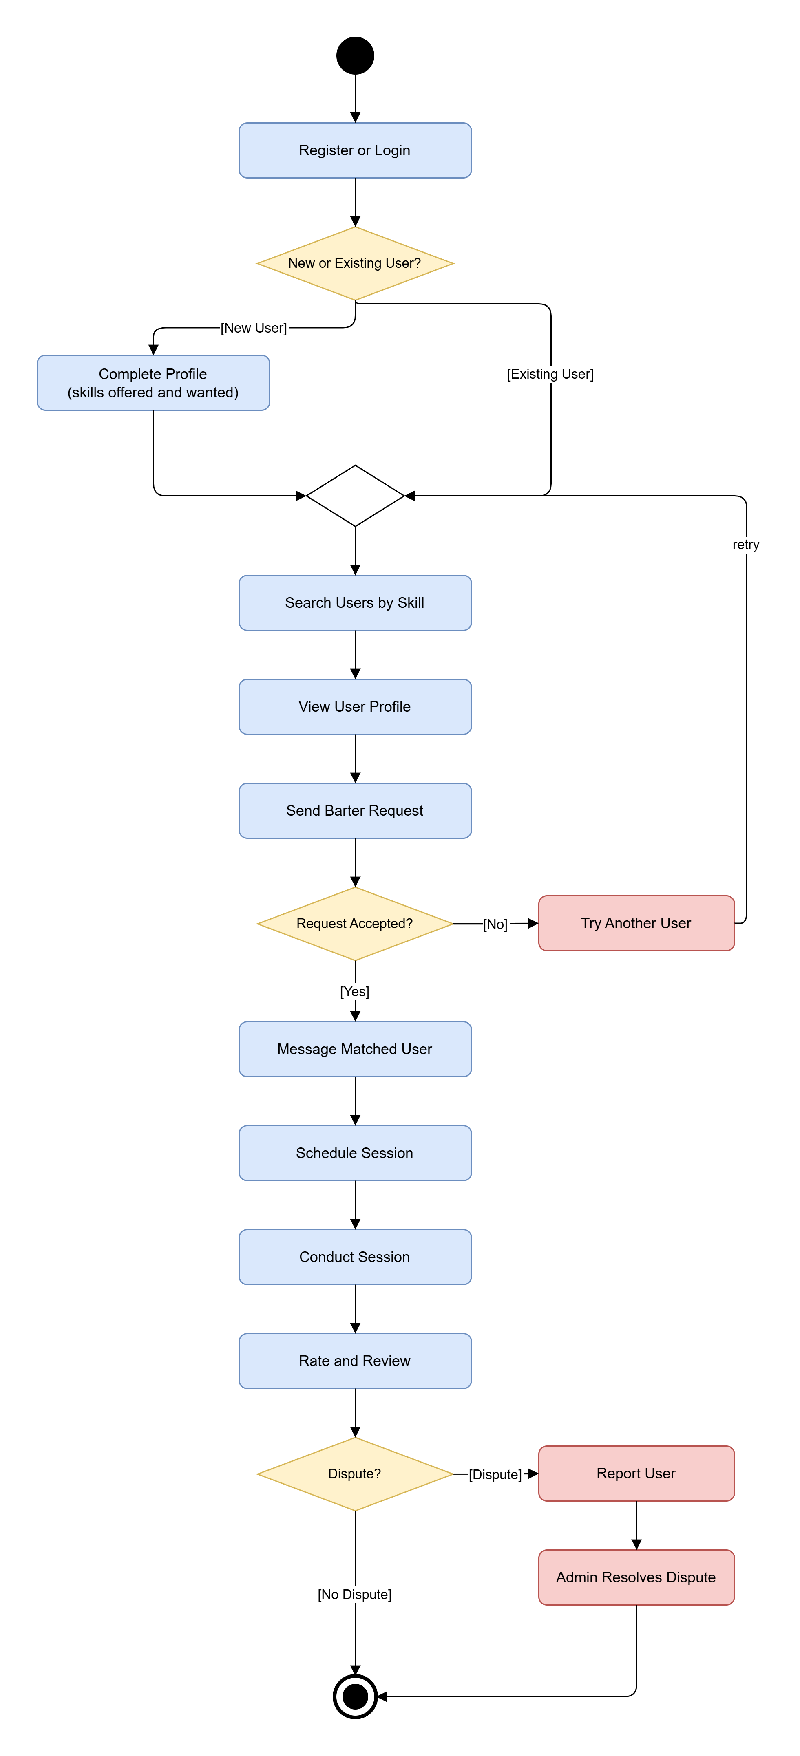
\includegraphics[page=1, width=0.62\textwidth]{diagrams.pdf}
\end{figure}

\newpage
\section{State Machine Diagram}
\vspace{4pt}

The diagram models the lifecycle of a Barter Request. It starts in Created, moves to Pending when sent, then branches four ways. Accepting moves it to Accepted, then Session Scheduled, then Session Completed, which is the only path to the final state. Rejecting moves it to Rejected. Cancelling moves it to Cancelled. No response in seven days moves it to Expired. Rejected, Cancelled, and Expired all connect to the final state. A scheduled session can also be cancelled by either party.

\begin{figure}[H]
\centering
\includegraphics[page=12, width=0.72\textwidth]{diagrams.pdf}
\end{figure}

%##########################################################
%  MILESTONE 3
%##########################################################
\newpage
\begin{center}
{\LARGE \textbf{Milestone 3: Design and Architecture}}\\[0.1cm]
\rule{\linewidth}{0.6mm}
\end{center}
\vspace{4pt}

\section{Architecture}
\vspace{4pt}

We used an N-Tier Layered Architecture. Each layer talks only to the one next to it. Microservices was too heavy for this scale. Event-driven was unnecessary since notifications are direct service calls. MVC principles are applied inside the Controller Layer only.

\subsection{Layer Breakdown}
\vspace{4pt}

\begin{longtable}{L{2.8cm} L{4.5cm} L{6.2cm}}
\toprule
\textbf{Layer} & \textbf{Components} & \textbf{Responsibility} \\
\midrule
\endfirsthead
\toprule
\textbf{Layer} & \textbf{Components} & \textbf{Responsibility} \\
\midrule
\endhead
\bottomrule
\endfoot
Presentation & Web Browser, Mobile App, Admin Dashboard & Renders the interface and collects user input. \\
Controller & Auth, Profile, Barter, Session, Admin, Notification Controllers & Validates input, checks permissions, routes to the correct service. \\
Business Logic & User Management, Skill Matching, Request Processing, Session Scheduling, Rating and Review, Dispute Resolution & Runs all core workflows and applies business rules. \\
Data Access & User, Skill, Barter, Session, Rating, Report Repositories & Wraps all database queries so business logic never writes raw queries. \\
Database & Users, Skills, Barter Requests, Sessions, Ratings, Reports & Stores all platform data. Only accessible through the Data Access Layer. \\
External Services & Email Server, SMS Gateway, Notification Service & Sends outbound notifications. Runs independently so a delivery failure does not affect core operations. \\
\bottomrule
\end{longtable}

\newpage
\section{Architecture Diagram}
\vspace{4pt}

\begin{figure}[H]
\centering
\includegraphics[page=2, width=\textwidth]{diagrams.pdf}
\end{figure}

\newpage
\section{Request Flow}
\vspace{4pt}

A barter request goes from the browser to the Barter Controller, which validates it and passes it to Business Logic. Request Processing checks eligibility, creates the request as Pending, and the Data Access Layer writes it to the database. Business Logic triggers the notification. The user sees a confirmation.

\section{Design Decisions}
\vspace{4pt}

\begin{longtable}{L{3.8cm} L{9.8cm}}
\toprule
\textbf{Decision} & \textbf{Reason} \\
\midrule
\endfirsthead
\toprule
\textbf{Decision} & \textbf{Reason} \\
\midrule
\endhead
\bottomrule
\endfoot
Repository Pattern & Business logic does not touch the database directly. Swapping the database engine only requires changes in the Data Access Layer. \\
Controller as Gatekeeper & Auth checks and input validation happen in one place. Invalid requests are blocked before reaching business logic. \\
External Services Isolated & A failed email does not crash a barter request. Core operations complete first, notification is separate. \\
Strict Layer Order & No layer skips another. Dependencies stay predictable and testable. \\
Role-Based Access Control & Admin and User roles are enforced at the Controller Layer. A regular user cannot reach admin functions. \\
\bottomrule
\end{longtable}

%##########################################################
%  MILESTONE 4
%##########################################################
\newpage
\begin{center}
{\LARGE \textbf{Milestone 4: Testing and Management}}\\[0.1cm]
\rule{\linewidth}{0.6mm}
\end{center}
\vspace{4pt}

\section{Test Plan}
\vspace{4pt}

We tested the platform across three levels. Unit tests target individual functions in isolation. Integration tests verify that two or more components work together correctly. System tests validate complete end-to-end flows against the functional requirements.

\subsection{Unit Tests}
\vspace{4pt}

\begin{longtable}{L{0.8cm} L{3cm} L{4cm} L{3.5cm} L{2.5cm}}
\toprule
\textbf{ID} & \textbf{Component} & \textbf{Test Case} & \textbf{Expected Result} & \textbf{Status} \\
\midrule
\endfirsthead
\toprule
\textbf{ID} & \textbf{Component} & \textbf{Test Case} & \textbf{Expected Result} & \textbf{Status} \\
\midrule
\endhead
\bottomrule
\endfoot
UT-01 & User Registration & Register with valid name, email, and password & Account created, user redirected to dashboard & Pass \\
UT-02 & User Registration & Register with an already existing email & System returns duplicate email error & Pass \\
UT-03 & User Login & Login with correct credentials & User authenticated and session started & Pass \\
UT-04 & User Login & Login with wrong password & Error shown, account locked after 3 attempts & Pass \\
UT-05 & Profile Management & Update skills offered and skills wanted & Profile saved and visible to other users & Pass \\
UT-06 & Profile Management & Save profile with empty required fields & System blocks save and shows validation error & Pass \\
UT-07 & Skill Search & Search for an existing skill & Matching user profiles returned & Pass \\
UT-08 & Skill Search & Search for a skill with no matches & No results message displayed & Pass \\
UT-09 & Barter Request & Send request with skill selected & Request created with Pending status & Pass \\
UT-10 & Barter Request & Send request without listing a skill & System prompts user to update profile first & Pass \\
UT-11 & Rating & Submit 5-star rating after completed session & Rating saved and displayed on profile & Pass \\
UT-12 & Rating & Skip written review and submit only stars & Stars saved, review field remains empty & Pass \\
\bottomrule
\end{longtable}

\subsection{Integration Tests}
\vspace{4pt}

\begin{longtable}{L{0.8cm} L{3.5cm} L{4cm} L{3cm} L{2.5cm}}
\toprule
\textbf{ID} & \textbf{Components} & \textbf{Test Case} & \textbf{Expected Result} & \textbf{Status} \\
\midrule
\endfirsthead
\toprule
\textbf{ID} & \textbf{Components} & \textbf{Test Case} & \textbf{Expected Result} & \textbf{Status} \\
\midrule
\endhead
\bottomrule
\endfoot
IT-01 & Auth + User DB & Register new user and verify record in database & User record stored with hashed password & Pass \\
IT-02 & Barter Request + Notification & Send barter request and verify recipient receives notification & Notification delivered to recipient & Pass \\
IT-03 & Barter Request + Barter DB & Accept request and verify status update in database & Status changed to Accepted in DB & Pass \\
IT-04 & Session + Notification & Schedule session and verify reminder notification sent & Reminder delivered to both users & Pass \\
IT-05 & Rating + Review DB & Submit rating after session and verify record stored & Rating record written to Review Database & Pass \\
IT-06 & Report + Admin Panel & User submits report and verify it appears in admin queue & Report visible in admin dispute queue & Pass \\
IT-07 & Auth + Controller & Unauthenticated user tries to access barter feature & Request blocked at Controller Layer & Pass \\
IT-08 & Admin + User DB & Admin suspends user and verify account status updated & User account marked suspended in database & Pass \\
\bottomrule
\end{longtable}

\subsection{System Tests}
\vspace{4pt}

\begin{longtable}{L{0.8cm} L{3cm} L{4.5cm} L{3cm} L{2.5cm}}
\toprule
\textbf{ID} & \textbf{Flow} & \textbf{Test Case} & \textbf{Expected Result} & \textbf{Status} \\
\midrule
\endfirsthead
\toprule
\textbf{ID} & \textbf{Flow} & \textbf{Test Case} & \textbf{Expected Result} & \textbf{Status} \\
\midrule
\endhead
\bottomrule
\endfoot
ST-01 & Full Barter Flow & User A registers, lists skill, finds User B, sends request, User B accepts, both schedule and complete session & Full flow completes without errors & Pass \\
ST-02 & Dispute Flow & User A files a report after session, Admin reviews and resolves with a warning & Report closed with resolution recorded & Pass \\
ST-03 & Expired Request & User A sends request, User B does not respond for 7 days & Request status changes to Expired automatically & Pass \\
ST-04 & Cancel Flow & User A cancels a pending request before recipient responds & Request status changes to Cancelled & Pass \\
ST-05 & Admin Management & Admin views all active sessions and suspends a flagged user & User suspended and sessions updated & Pass \\
ST-06 & Rating Flow & Both users rate each other after a completed session & Ratings saved and both profile scores updated & Pass \\
\bottomrule
\end{longtable}

\newpage
\section{Version Control}
\vspace{4pt}

We used GitHub for version control throughout the project. All documentation files, diagrams, and LaTeX source files were committed across multiple commits. The repository is available at 
\url{https://github.com/JunaidAhmed13/skill-barter-platform}

\begin{figure}[H]
\centering
\includegraphics[page=9, width=\textwidth]{diagrams.pdf}
\end{figure}

\begin{figure}[H]
\centering
\includegraphics[page=4, width=\textwidth]{diagrams.pdf}
\end{figure}

\newpage
\section{Project Planning}
\vspace{4pt}

\subsection{Gantt Chart}
\vspace{4pt}

Milestone 1 tasks ran through Week 1. Milestone 2 modeling work ran through Weeks 2 and 3. Milestone 3 architecture work ran through Week 3. Milestone 4 testing and documentation was completed in Week 4.

\begin{figure}[H]
\centering
\includegraphics[page=8, width=\textwidth]{diagrams.pdf}
\end{figure}

\subsection{PERT Chart}
\vspace{4pt}

Total project duration is 10 working days. The critical path runs through Functional Requirements (3 days), Behavioral Diagrams (4 days), and Architecture Design (3 days). Non-critical tasks including Class Diagram, UML Refinement, and Context and DFD carry 1 to 2 days of slack each.

\begin{figure}[H]
\centering
\includegraphics[page=10, width=\textwidth]{diagrams.pdf}
\end{figure}

\newpage
\section{Risk Analysis}
\vspace{4pt}

\begin{longtable}{L{0.6cm} L{3.2cm} L{1.8cm} L{1.8cm} L{1.8cm} L{4cm}}
\toprule
\textbf{ID} & \textbf{Risk} & \textbf{Likelihood} & \textbf{Impact} & \textbf{Priority} & \textbf{Mitigation} \\
\midrule
\endfirsthead
\toprule
\textbf{ID} & \textbf{Risk} & \textbf{Likelihood} & \textbf{Impact} & \textbf{Priority} & \textbf{Mitigation} \\
\midrule
\endhead
\bottomrule
\endfoot
R-01 & Incomplete requirements & Medium & High & High & Review requirements with all team members before moving to modeling \\
R-02 & Diagram errors or inconsistencies & High & Medium & High & Peer review all diagrams before submission \\
R-03 & Uneven workload distribution & Medium & Medium & Medium & Assign tasks at the start of each milestone with clear deadlines \\
R-04 & Version conflicts in documentation & Low & Medium & Medium & Use GitHub branches and commit frequently \\
R-05 & Scope creep in documentation & Medium & Low & Low & Stick to the assignment brief \\
R-06 & Tool unavailability & Low & High & Medium & Keep local backups of all files and diagrams \\
R-07 & Misunderstanding of SE notation & Medium & High & High & Reference Sommerville and IEEE standards before drawing diagrams \\
R-08 & Late submission due to review delays & Low & High & High & Complete each milestone two days before the deadline \\
\bottomrule
\end{longtable}

\section{Team Roles}
\vspace{4pt}

\textbf{Muhammad Sadiq Aslam Khan} (01-134242-091) -- Milestone 2: Context Diagram, DFD Level 1 and Level 2, Class Diagram, Sequence Diagram, architecture design, GitHub repository management.

\textbf{Malik Junaid Ahmed} (01-134242-061) -- Milestone 1: Functional and non-functional requirements, use case description tables. Milestone 4: Test plan, Gantt chart, PERT chart, risk analysis, team roles.

\textbf{Bilawal Khokhar} (01-134242-036) -- Milestone 3: UML refinement, state machine diagram, layered architecture documentation.

\textbf{Shah Murad} (01-134242-113) -- Milestone 1: Problem statement, project scope, use case diagrams. Milestone 2: Activity diagram, state machine diagram.

\end{document}